\chapter{Evaluierung} \label{cha:Evaluierung}

In diesem Kapitel soll der zuvor implementierte Verfahren evaluiert werden.  lassen sich eine Reihe von Testanalysen durchführen, um die Methode auf die Genauigkeit und die Leistungsfähigkeit zu testen.


\section{Evaluierung der 1.Verfahren}

Hier wird das 1. Verfahren mit dessen Genauigkeit und Leistunsfähigkeit evaluiert. Als in Kapital 3 vorstellt, diese Methode ist häuptlich für den Fall, bei der Aufnahmen die Smartphone in der Hand gehalten. Dann brauchen eine Bildregistration Operation, um die Bildern in dasselbe Korordinatensystem zu transformieren. Die Funktion dieses Moduls wirkt sich direkt auf die Entstehung der Differenzbildern aus und hat einen wesentlichen Einfluss auf die spätere Erkennung, insbesondere die Erkennung von QR-Mustern. Deswegen wird eine Analysierung dafür durchgeführt.

Um die Leistung visuell zu verstehen, wird einen Satz Parameter gesetzt. Das Modulationsamplitude erstellt als 6, Datenblock als $ 4 \times 4 Pixel$, QR Muster Größe als $ 72 \times 72 Pixel $.  In der Rhein von Bildern wird das erste Bild und das letzte Bild verglichen, wie in Abbildung \ref{fig:vorregistration} zeigt. 


%Die durchschnittliche Entfernung der entsprechenden Pixel zwischen den zwei Bildern beträgt ca.2 Pixel. 
%Abbildung \ref{fig:nachregis} zeigt das Bild nach der Bildregistration. Wie zu sehen ist, ist der Abstand gut komprimiert. %Die durchschnittliche Entfernung hier beträgt ca. 0.45 Pixel.

\begin{figure}[H]
 \centering 
  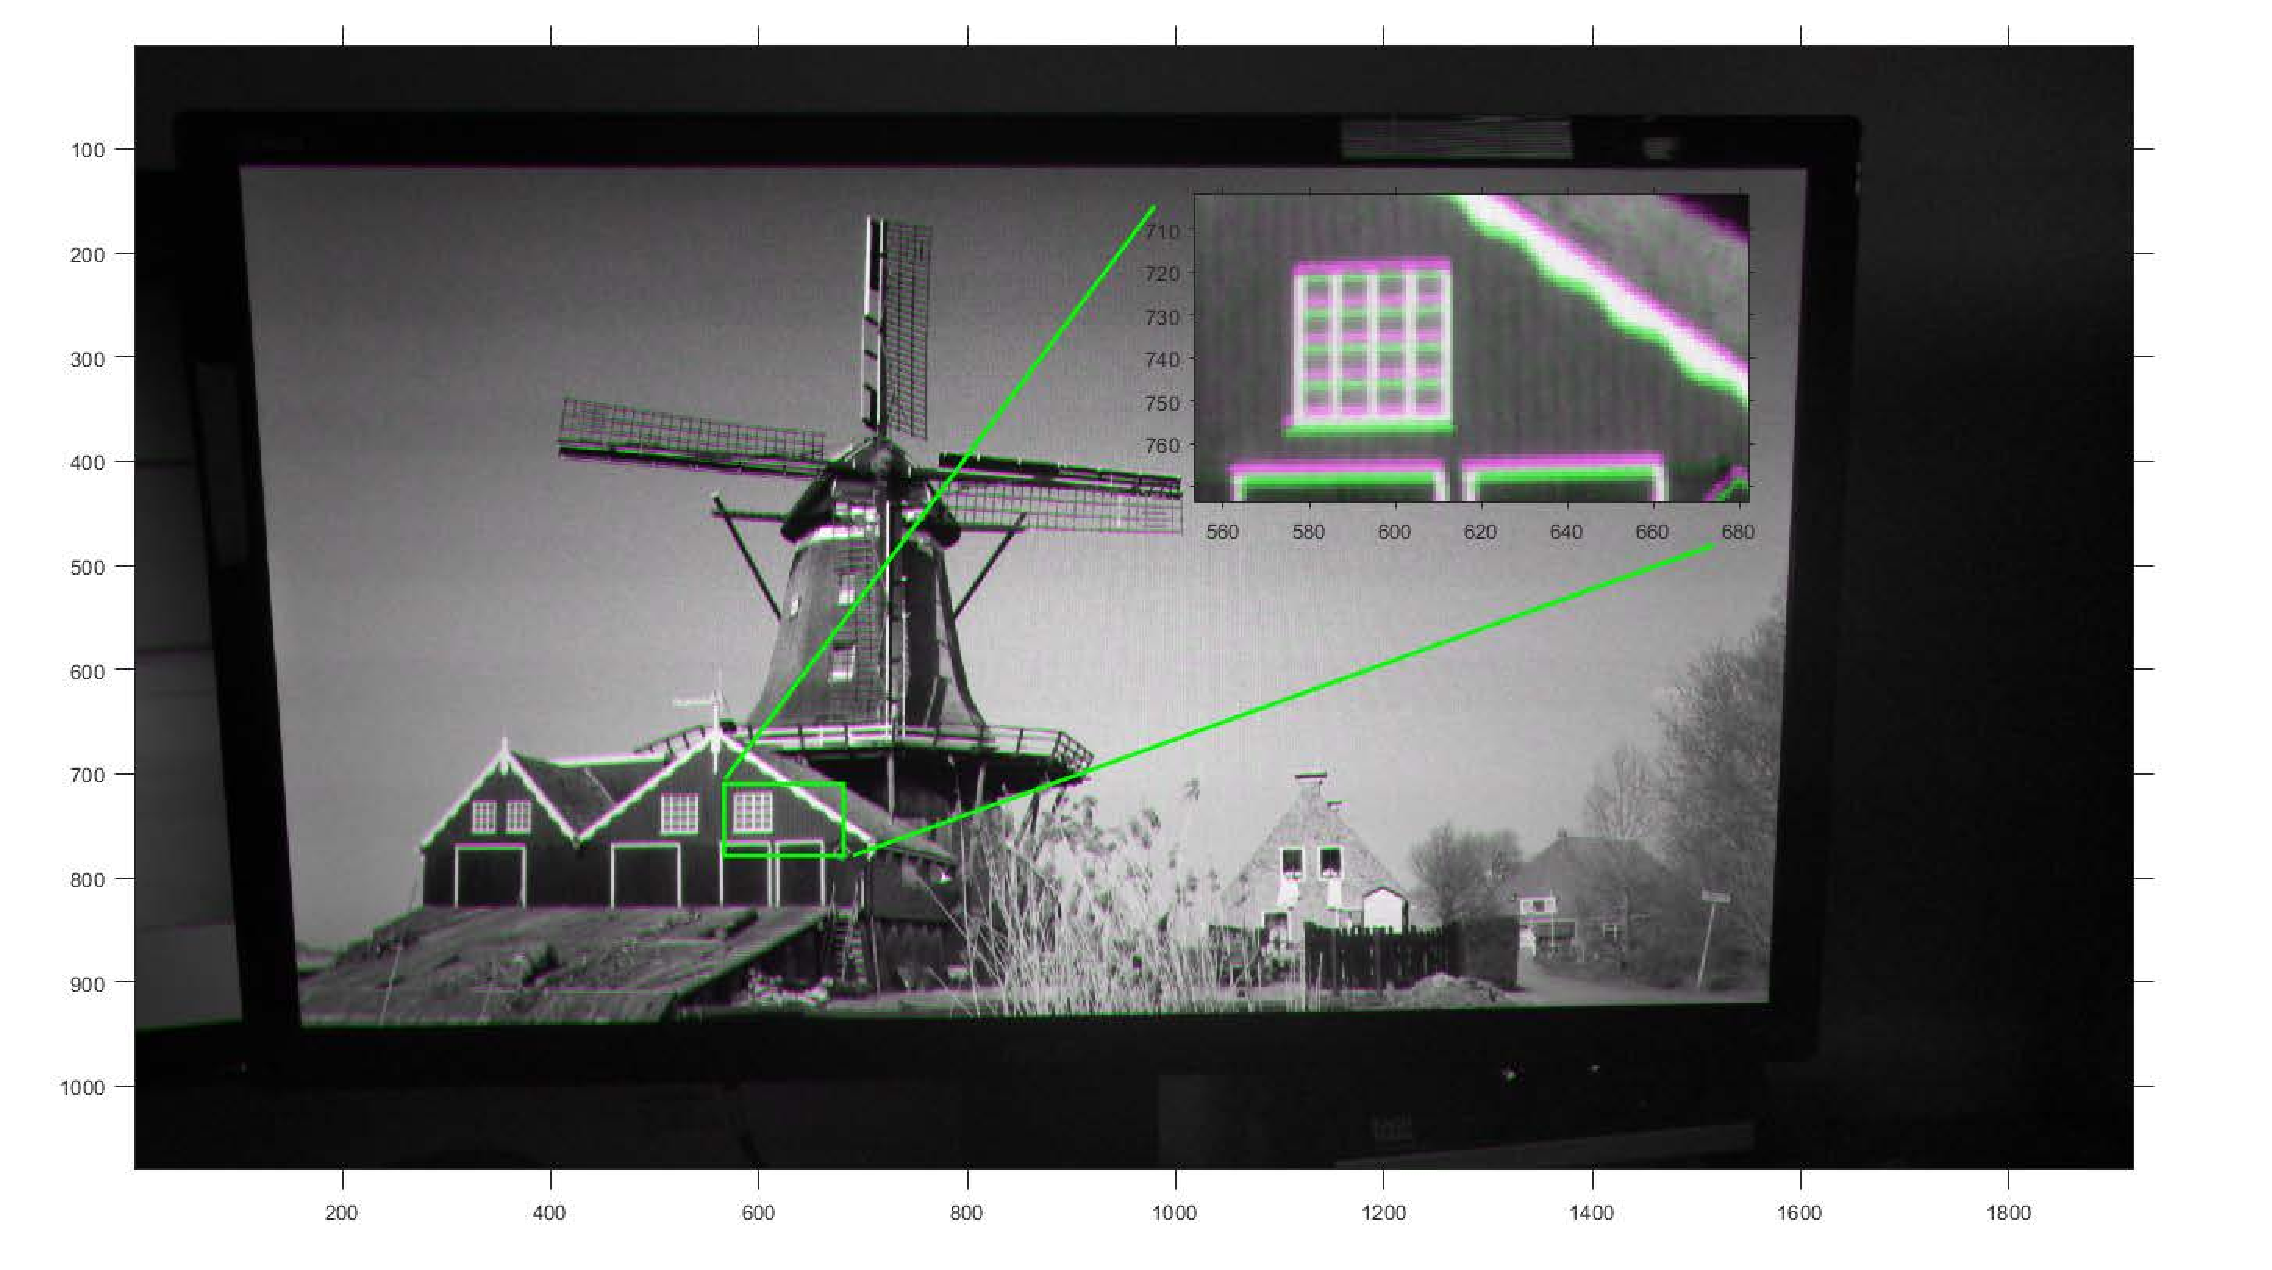
\includegraphics[keepaspectratio,width=1.0\textwidth]{images/5_Implementirung/vorregistration.pdf}
 \caption{Verschiebung durch Handshake}
 \label{fig:vorregistration}
\end{figure}

Aus der Abbildung ist deutlich zu erkennen, dass das Bild durch Handshake eine deutliche Verschiebung erfahren hat. Durch die Bildregistration, die in dieser Arbeit vorstellt, kann dieses Problem effektive gelöst werden. Abbildung \ref{fig:Konvergenzkurve} zeigt die Konvergenzkurve des Fehlers J bei der Summenwertbildung im Quadrat aller Korrespondenzpunkte.

\begin{figure}[H]
 \centering 
  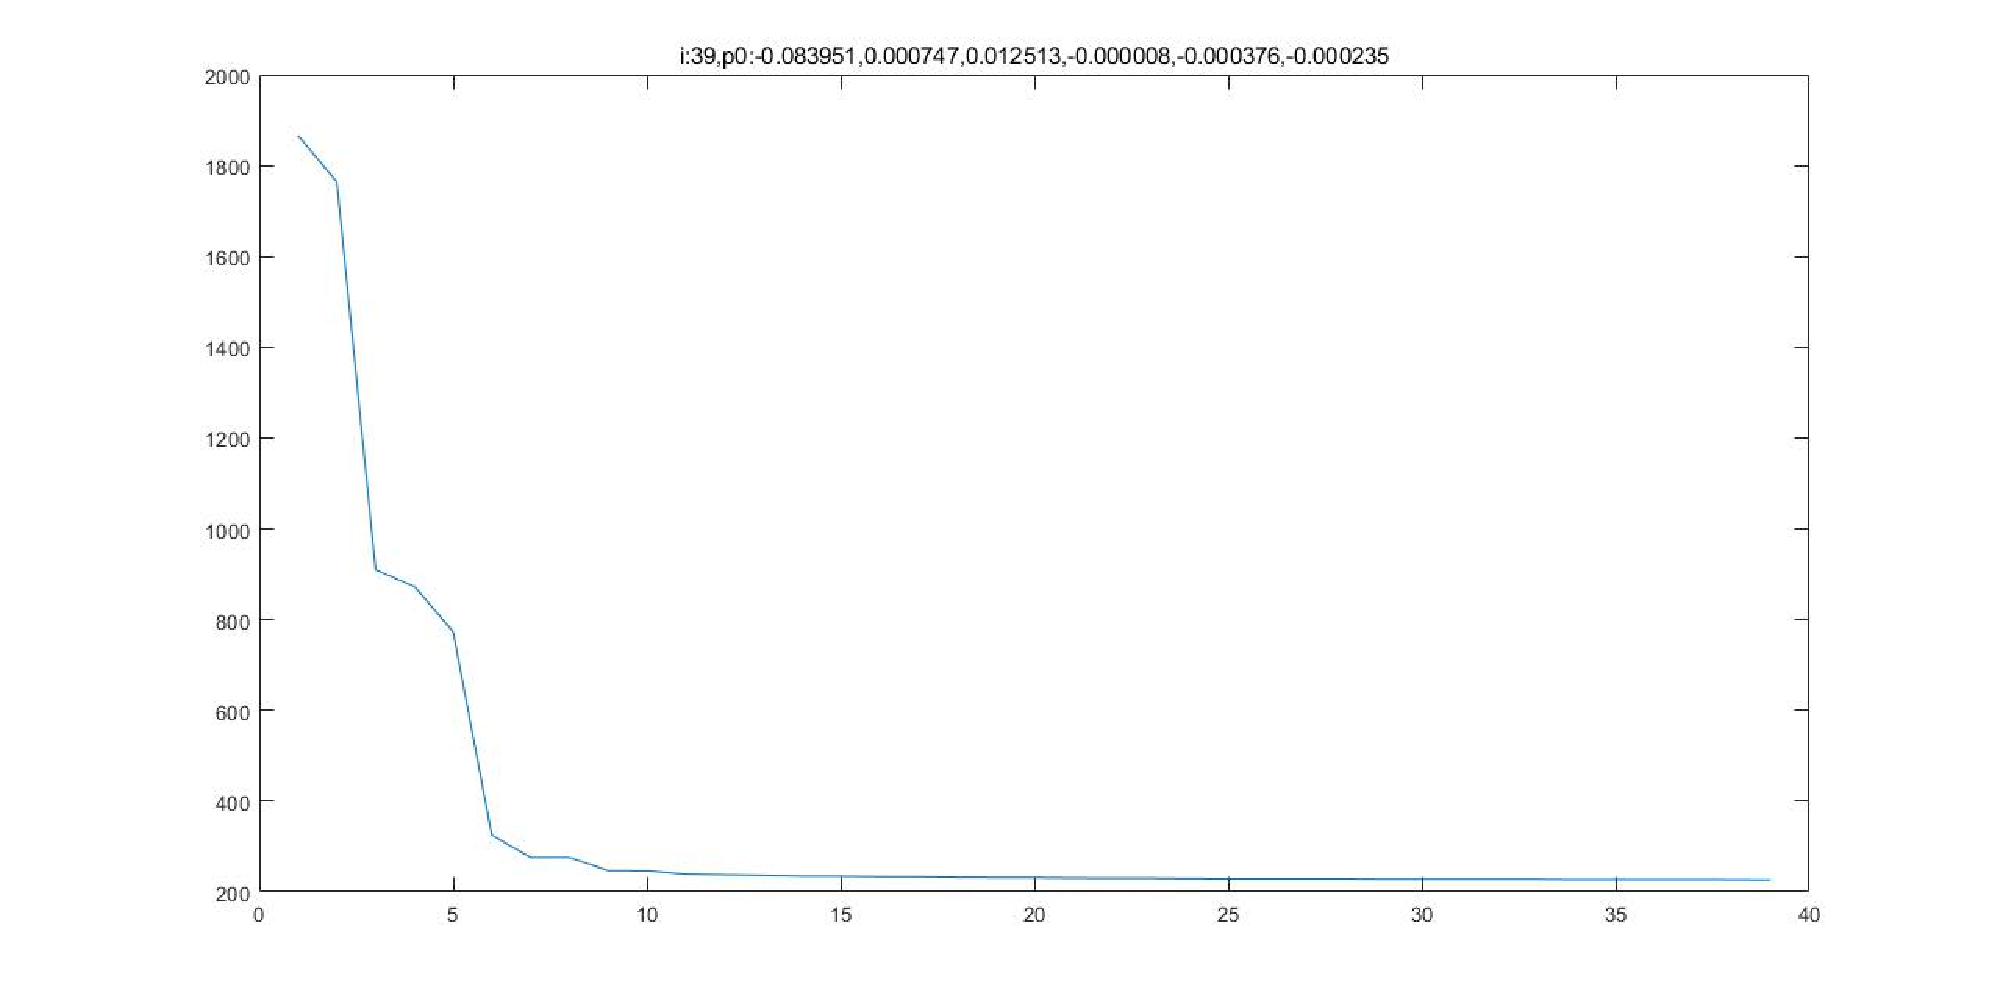
\includegraphics[keepaspectratio,width=1.0\textwidth]{images/6_Auswertung/J8.pdf}
 \caption{Konvergenzkurve von J}
 \label{fig:Konvergenzkurve}
\end{figure}

Die vertikale Koordinate repräsentiert den Fehlerwert J und die horizontale Koordinate repräsentiert die Anzahl der Iterationen des Algorithmus. Als zeigt in der Abbildung, wird J nach etwa 10 Iterationen konvergiert. Die konkreten Daten wird in Tabelle \ref{tbl:Daten des Fehlers} gezeigt.

\begin{table}[htb]
	\captionabove{Daten des Fehlers}
	\label{tbl:Daten des Fehlers}
	\footnotesize
	\centering
	\rowcolors{2}{white}{gray!25}	%TUgreen!25
	%\begin{tabular}{|p{2cm}|p{4cm}|p{3cm}|p{3cm}|}	%p{}m{}b{}clr
	\begin{tabular}{|c|c|c|c|c|c|}
	\toprule
	\textbf{Verglicht Bilder} & \textbf{Anzahl der Punkt} & \textbf{Ursprünglich Fehler} & \textbf{Mittelwert} &\textbf{Ergebnis Fehler} & \textbf{Mittelwert}\\
	\midrule
	1-2 & 849 & 350.5674 & 0.4129 & 224.9265 & 0.2649\\ 
	1-3 & 723 & 826.8834 & 1.1437 & 236.0301 & 0.3265\\ 
	1-4 & 619 & 662.3621 & 1.0701 & 208.4760 & 0.3368\\ 
	1-5 & 500 & 723.2307 & 1.4465 & 207.1174 & 0.4142\\ 
	1-6 & 835 & 1607.4002 & 1.9250& 231.7138 & 0.2775\\ 
	1-7 & 802 & 1059.4579 & 1.3210& 260.3104 & 0.3246\\ 
	1-8 & 803 & 1863.9972 & 2.3213& 246.7970 & 0.3073\\ 
	\bottomrule
	\end{tabular}
\end{table} 

Abbildung \ref{fig:Bild nach Registration} zeigt das Bild nach der Bildregistration. Wie zu sehen ist, ist der Feler gut komprimiert.
\begin{figure}[H]
 \centering 
  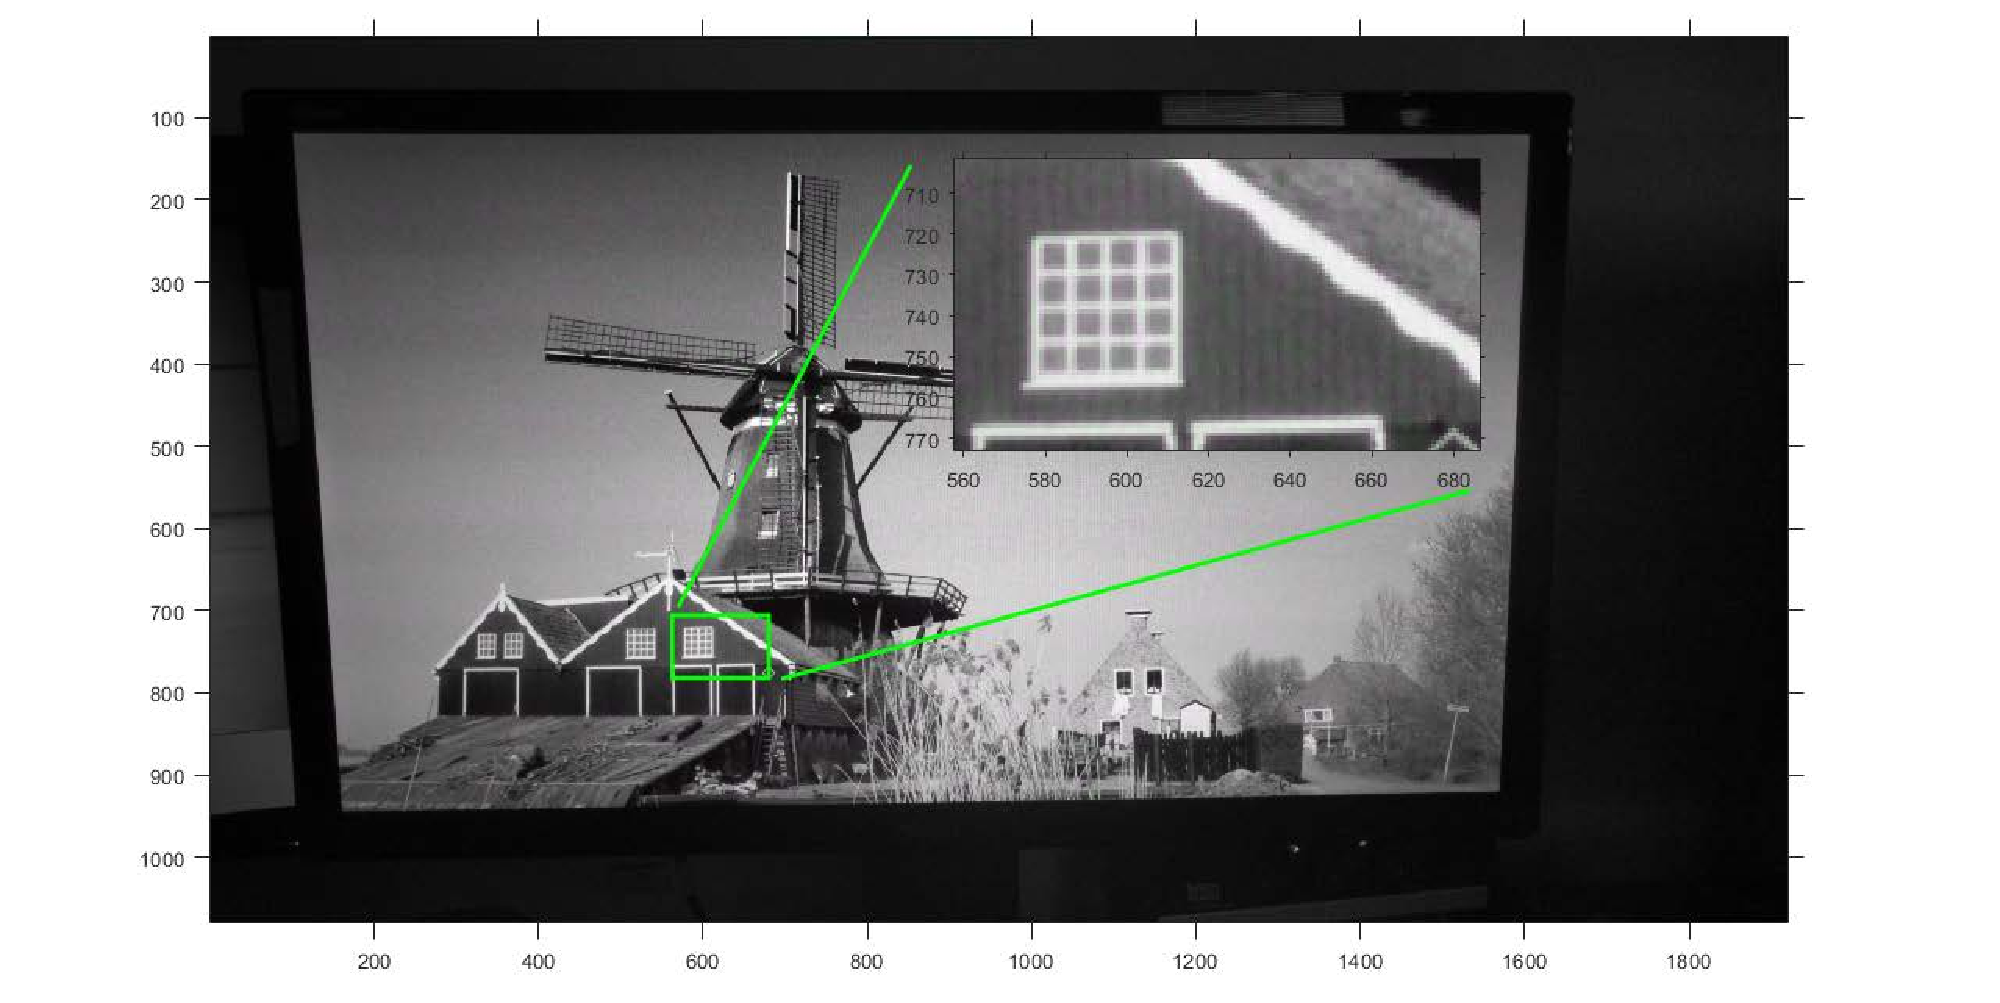
\includegraphics[keepaspectratio,width=1.05\textwidth]{images/5_Implementirung/nachregis.pdf}
 \caption{Bild nach Registration}
 \label{fig:Bild nach Registration}
\end{figure}


\section{Evaluierung der vorhandenen Funktionalität}